\documentclass[12pt, a4paper]{article}
\usepackage[utf8]{inputenc}
\usepackage[T1]{fontenc}
\usepackage{ngerman}
\usepackage{amsmath, amssymb, amsthm}
\usepackage{mathtools}
\usepackage{bm}
\usepackage{graphicx}
\usepackage{xcolor}
\usepackage{pgfplots}
\pgfplotsset{compat=1.18}
\usepackage{tikz}
\usetikzlibrary{arrows.meta, positioning, shapes.geometric, calc,
                decorations.pathreplacing, matrix, fit, backgrounds}
\usepackage{booktabs}
\usepackage{array}
\usepackage{longtable}
\usepackage{geometry}
\usepackage{setspace}
\usepackage{parskip}
\usepackage{hyperref}
\usepackage{cleveref}
\usepackage{natbib}
\usepackage{caption}
\usepackage{subcaption}
\usepackage{algorithm}
\usepackage{algpseudocode}
\usepackage{enumitem}
\usepackage{multirow}
\usepackage{float}
\usepackage{rotating}
\usepackage{microtype}
\setlist[itemize,1]{label=--}

\geometry{margin=2.5cm}

% ---------- Farben ----------
\definecolor{mainblue}{RGB}{25, 70, 140}
\definecolor{accentred}{RGB}{180, 50, 30}
\definecolor{lightgray}{RGB}{245, 245, 248}
\definecolor{darkgray}{RGB}{60, 60, 70}
\definecolor{darkgreen}{RGB}{30, 100, 50}
\definecolor{darkorange}{RGB}{200, 100, 0}

% ---------- Theorem-Umgebungen ----------
\newtheorem{theorem}{Theorem}[section]
\newtheorem{lemma}[theorem]{Lemma}
\newtheorem{proposition}[theorem]{Proposition}
\newtheorem{corollary}[theorem]{Korollar}
\theoremstyle{definition}
\newtheorem{definition}[theorem]{Definition}
\newtheorem{example}[theorem]{Beispiel}
\theoremstyle{remark}
\newtheorem{remark}[theorem]{Bemerkung}

% ---------- Hyperref ----------
\hypersetup{
  colorlinks=true,
  linkcolor=mainblue,
  citecolor=accentred,
  urlcolor=mainblue,
  pdftitle={Äquivalenz durch Sicht: Graphische Deduktion und die Überflüssigkeit der Matrix},
  pdfauthor={Stephan Epp},
}

% ---------- Makros ----------
\newcommand{\R}{\mathbb{R}}
\newcommand{\C}{\mathbb{C}}
\newcommand{\N}{\mathbb{N}}
\newcommand{\Z}{\mathbb{Z}}
\newcommand{\vx}{\bm{x}}
\newcommand{\vu}{\bm{u}}
\newcommand{\vy}{\bm{y}}
\newcommand{\vA}{\bm{A}}
\newcommand{\vB}{\bm{B}}
\newcommand{\vC}{\bm{C}}
\newcommand{\vP}{\bm{P}}
\newcommand{\vQ}{\bm{Q}}
\newcommand{\vI}{\bm{I}}
\newcommand{\vV}{\bm{V}}
\newcommand{\vLambda}{\bm{\Lambda}}
\newcommand{\vK}{\bm{K}}
\newcommand{\vR}{\bm{R}}
\newcommand{\vG}{\bm{G}}
\newcommand{\vS}{\bm{S}}
\newcommand{\vSigma}{\bm{\Sigma}}
\newcommand{\vD}{\bm{D}}
\newcommand{\vL}{\bm{L}}
\newcommand{\vT}{\bm{T}}
\newcommand{\T}{\top}
\newcommand{\tr}{\mathrm{tr}}
\newcommand{\rank}{\mathrm{rank}}
\newcommand{\spec}{\sigma}
\newcommand{\re}{\mathrm{Re}}
\newcommand{\im}{\mathrm{Im}}
\newcommand{\diag}{\mathrm{diag}}
\newcommand{\Ver}{\mathrm{Ver}}
\newcommand{\Knot}{\mathrm{Knot}}
\newcommand{\Kant}{\mathrm{Kant}}
\newcommand{\Graph}{\mathcal{G}}
\newcommand{\Ded}{\mathrm{Ded}}
\newcommand{\Ind}{\mathrm{Ind}}

\title{\textbf{Äquivalenz durch Sicht}\\[0.5em]
  {\Large\itshape Graphische Deduktion und die fundamentale Überflüssigkeit\\ der Matrix in algebraischen Beweisen}}
\author{Stephan Epp}
\date{15. September 2026}

% ============================================================
\begin{document}
% ============================================================

\maketitle
\tableofcontents
\newpage

% ============================================================
\section{Einleitung}
\label{sec:einleitung}
% ============================================================

Wie kann man Verbundenheit oder Äquivalenz oder dieselbe Darstellung besser vergleichen, als dass man das eine in einer formalen mathematischen Beweisführung, welches bisher immer genutzt worden ist, nie wieder betrachtet und vollständig darauf verzichtet? Das hat zur Konsequenz, dass Matrizen nie wieder verwendet werden in mathematischen Beweisen der Algebra, sondern nur noch Graphen. Der erste Graph, den es gibt, ist der Graph mit zwei Knoten und einer Kante verbunden. Einfacher geht es nicht und weniger geht auch nicht, denn sonst ist es kein Graph mehr. Sofort ist klar, dass dieser Graph die zwei kreuz zwei Matrix repräsentiert, die kleinste, die es gibt. Damit würdigen wir immer mehr die Darstellung der Matrix, indem wir auf sie verzichten und Beweise und Anschauungen nur noch mit Graphen durchführen. Denn allen ist klar, wir verzichten damit auf Matrizen und vermissen sie sogar schon, denn vielleicht ist der ein oder andere Beweis jetzt sogar etwas mühsamer. Aber halt! Die Äquivalenz verbietet uns Matrizen zu nutzen. Deshalb bleiben wir vollständig und immer nur noch bei Graphen und führen Beweise weiter konsequent selbst in den kompliziertesten Aussagen über dieselben.

Das Prinzip der Deduktion oder des Beweisens durch Deduktion hat den bekannten Anfang so wie beim Induktionsbeweis. Im Schritt aber wird dann das Element $n$ gewählt, und dann von $n$ nach $n-1$ argumentiert und so die Behauptung angewendet auf $n-1$. Erst die Deduktion ist die Beweismethode die die Methode der Wahl ist gegenüber der vollständigen Induktion. Die vollständige Induktion argumentiert über alle Elemente bis ins Unendliche. Das aber ist bei Graphen und bei Matrizen nie der Fall. Wer die Induktion angewandt hat und dies als Beweis geglaubt hat, der hat sehr dumm gehandelt. Denn er hat übersehen, dass diese Beweisführung gar keine Beweisführung ist. Es wurde eine Methode angewendet, bei der man sicher wusste, es wird ja zu viel gezeigt. Aber das macht es nicht besser. Da wurde zu viel gezeigt und damit nicht genau das, was gezeigt werden muss. Denn ein Beweis ist erst dann ein Beweis, wenn er genau das zeigt, was gezeigt werden muss. Aber genau das impliziert nicht zu viel und nicht zu weniel.

\subsection{Wissenschaftliche Einordnung}
\label{subsec:einordnung}

Die vorliegende Arbeit behandelt drei zentrale Themenkomplexe:

\begin{enumerate}[label=(\roman*)]
  \item \textbf{Äquivalenzprinzip und graphische Darstellung:} Formaler mathematischer Nachweis, dass die Darstellung algebraischer Strukturen mittels Graphen äquivalent zur Matrixdarstellung ist, und dass diese Äquivalenz es rechtfertigt, vollständig auf Matrizen zu verzichten.

  \item \textbf{Minimale graphische Basis:} Rigoroser Beweis, dass der einfachste nichtleere Graph -- bestehend aus zwei Knoten und einer Kante -- die fundamentale Basisstruktur darstellt, aus welcher alle komplexeren Strukturen ableitbar sind, und dass dieser Graph exakt der $2 \times 2$ Matrix entspricht.

  \item \textbf{Deduktion versus Induktion:} Kritische Analyse und formale Beweisenführung, dass die deduktive Methode die einzige mathematisch legitime Beweismethode darstellt, während die vollständige Induktion methodisch fehlerhaft ist, da sie zu viel zeigt und damit nicht exakt das zeigt, was gezeigt werden muss.
\end{enumerate}

\subsection{Aufbau der Arbeit}
\label{subsec:aufbau}

Abschnitt~\ref{sec:grundlagen} legt die formalen Grundlagen der Graphentheorie und der Äquivalenzrelationen fest. Abschnitt~\ref{sec:minimalegraph} beweist, dass der Zwei-Knoten-Graph die minimale nichtleere Struktur darstellt. Abschnitt~\ref{sec:aequivalenzprinzip} beweist die strukturelle Äquivalenz zwischen Graphen und Matrizen. Abschnitt~\ref{sec:deduktion} entwickelt die Deduktion als einzig legitime Beweismethode und kritisiert die Induktion. Abschnitt~\ref{sec:graphische_beweise} zeigt, wie alle algebraischen Sätze rein graphisch mit deduktiven Methoden bewiesen werden. Abschnitt~\ref{sec:ausblick} enthält einen umfassenden Ausblick und offene Forschungsfragen.

% ============================================================
\section{Mathematische Grundlagen und Definitionen}
\label{sec:grundlagen}
% ============================================================

\subsection{Graphen und ihre Elementarstruktur}
\label{subsec:graphentheorie}

\begin{definition}[Ungerichteter Graph]
\label{def:graph}
Ein \emph{ungerichteter Graph} ist ein Paar $\Graph = (V, E)$, wobei:
\begin{enumerate}[label=(\alph*)]
  \item $V$ eine nichtleere, endliche Menge ist, deren Elemente \emph{Knoten} oder \emph{Vertizes} genannt werden.
  \item $E \subseteq \{\{u, v\} : u, v \in V, u \neq v\}$ eine Menge von ungerichteten Kanten ist, wobei jede Kante eine zweielementige Teilmenge von $V$ darstellt.
\end{enumerate}
Für einen Graphen $\Graph = (V, E)$ schreiben wir $|V|$ für die Anzahl der Knoten und $|E|$ für die Anzahl der Kanten.
\end{definition}

\begin{definition}[Gerichteter Graph]
\label{def:digraph}
Ein \emph{gerichteter Graph} (oder \emph{Digraph}) ist ein Paar $\Graph = (V, E)$, wobei:
\begin{enumerate}[label=(\alph*)]
  \item $V$ eine nichtleere, endliche Menge von Knoten ist.
  \item $E \subseteq V \times V$ eine Menge von \emph{gerichteten Kanten} ist, wobei jede Kante ein geordnetes Paar $(u, v)$ mit $u, v \in V$ darstellt.
\end{enumerate}
Eine Kante $(v, v)$ heißt \emph{Schleife} oder \emph{Loop}.
\end{definition}

\begin{definition}[Gewichteter Graph]
\label{def:gewichteter_graph}
Ein \emph{gewichteter Graph} ist ein Tripel $\Graph = (V, E, w)$, wobei:
\begin{enumerate}[label=(\alph*)]
  \item $(V, E)$ ein gerichteter Graph ist.
  \item $w: E \to \R$ eine Gewichtsfunktion ist, die jeder Kante $(u, v) \in E$ ein Gewicht $w(u, v) \in \R$ zuweist.
\end{enumerate}
\end{definition}

\begin{definition}[Minimalität eines Graphen]
\label{def:minimalitaet}
Ein Graph $\Graph = (V, E)$ heißt \emph{minimal nichtleer}, wenn die folgenden Bedingungen erfüllt sind:
\begin{enumerate}[label=(\alph*)]
  \item $|V| \geq 1$ und $|E| \geq 1$ (der Graph ist nichtleer).
  \item Für jeden echten Teilgraphen $\Graph' = (V', E')$ mit $\Graph' \neq \Graph$ gilt: Wenn $V' \subsetneq V$, dann $E' = \emptyset$ oder $\Graph'$ ist nicht zusammenhängend.
  \item Die Entfernung einer beliebigen Kante führt zu einem Graphen, der nicht zusammenhängend ist.
\end{enumerate}
\end{definition}

\begin{definition}[Adjazenzmatrix]
\label{def:adjazenzmatrix}
Für einen gewichteten gerichteten Graphen $\Graph = (V, E, w)$ mit $V = \{v_1, \ldots, v_n\}$ ist die \emph{Adjazenzmatrix} $\vA_{\Graph} \in \R^{n \times n}$ definiert als:
\[
  (\vA_{\Graph})_{ij} = \begin{cases}
    w(v_i, v_j) & \text{falls } (v_i, v_j) \in E \\
    0 & \text{falls } (v_i, v_j) \notin E
  \end{cases}
\]
\end{definition}

\subsection{Äquivalenzrelationen und isomorphe Darstellungen}
\label{subsec:aequivalenz}

\begin{definition}[Äquivalenzrelation]
\label{def:aequivalenz}
Eine Relation $\sim$ auf einer Menge $S$ heißt \emph{Äquivalenzrelation}, wenn sie folgende Eigenschaften erfüllt:
\begin{enumerate}[label=(\alph*)]
  \item \emph{Reflexivität:} Für alle $a \in S$ gilt $a \sim a$.
  \item \emph{Symmetrie:} Für alle $a, b \in S$ gilt: Wenn $a \sim b$, dann $b \sim a$.
  \item \emph{Transitivität:} Für alle $a, b, c \in S$ gilt: Wenn $a \sim b$ und $b \sim c$, dann $a \sim c$.
\end{enumerate}
\end{definition}

\begin{definition}[Graphisomorphismus]
\label{def:graphisomorphismus}
Seien $\Graph_1 = (V_1, E_1)$ und $\Graph_2 = (V_2, E_2)$ zwei ungerichtete Graphen. Ein \emph{Graphisomorphismus} ist eine Bijektion $\phi: V_1 \to V_2$ mit der Eigenschaft:
\[
  \{u, v\} \in E_1 \iff \{\phi(u), \phi(v)\} \in E_2
  \quad \text{für alle } u, v \in V_1
\]
Wenn es einen Graphisomorphismus zwischen $\Graph_1$ und $\Graph_2$ gibt, schreiben wir $\Graph_1 \cong \Graph_2$ und sagen, die Graphen sind \emph{isomorph}.
\end{definition}

\begin{definition}[Strukturelle Äquivalenz]
\label{def:struktur_aequivalenz}
Zwei mathematische Strukturen $\mathcal{S}_1$ und $\mathcal{S}_2$ heißen \emph{strukturell äquivalent}, notiert $\mathcal{S}_1 \approx \mathcal{S}_2$, wenn es eine Bijektion zwischen ihren Elementen gibt, die alle definierten Operationen und Relationen erhält. Das heißt, jede mathematische Aussage über $\mathcal{S}_1$ kann in eine äquivalente Aussage über $\mathcal{S}_2$ übersetzt werden und umgekehrt.
\end{definition}

% ============================================================
\section{Der minimal-nichtleere Graph als fundamentale Basis}
\label{sec:minimalegraph}
% ============================================================

\subsection{Charakterisierung und Eindeutigkeit}
\label{subsec:minimal_charakterisierung}

\begin{lemma}[Minimalität und Zusammenhang]
\label{lem:minimal_zusammenhang}
Ein Graph $\Graph = (V, E)$ ist minimal nichtleer genau dann, wenn $|V| = 2$, $|E| = 1$, und die beiden Knoten durch die einzige Kante verbunden sind.
\end{lemma}

\begin{proof}
Wir zeigen beide Richtungen.

\textbf{($\Rightarrow$)} Angenommen, $\Graph = (V, E)$ ist minimal nichtleer. Dann gelten nach Definition~\ref{def:minimalitaet}:
\begin{enumerate}[label=(\roman*)]
  \item $|V| \geq 1$ und $|E| \geq 1$.
  \item Für jeden echten Teilgraphen $\Graph'$ mit $V' \subsetneq V$ gilt: $\Graph'$ ist nicht zusammenhängend.
  \item Die Entfernung einer beliebigen Kante führt zu Unzusammenhang.
\end{enumerate}

Angenommen, $|V| \geq 3$. Dann können wir eine Partition $V = V_1 \cup V_2$ mit $V_1, V_2 \neq \emptyset$ und $V_1 \cap V_2 = \emptyset$ wählen. Der Teilgraph $\Graph_1 = (V_1, E_1)$ mit $E_1 = E \cap (V_1 \times V_1)$ hat $|V_1| < |V|$. Nach Bedingung (ii) muss $\Graph_1$ unzusammenhängend sein. Dies bedeutet, dass es keine Kanten zwischen $V_1$ und $V_2$ gibt, also $E \subseteq (V_1 \times V_1) \cup (V_2 \times V_2)$.

Betrachten wir nun die Entfernung jeder Kante in $E$. Nach Bedingung (iii) führt dies zu Unzusammenhang. Aber wenn wir eine Kante $(u, v)$ mit $u, v \in V_1$ entfernen, bleiben alle Kanten zwischen $V_2$ und $V_2$ erhalten. Der resultierende Graph bleibt innerhalb von $V_2$ zusammenhängend -- ein Widerspruch zu Bedingung (iii), falls $E \cap (V_2 \times V_2) \neq \emptyset$.

Also müssen wir $|V| = 2$ haben. Sei $V = \{u, v\}$.

Angenommen, $|E| \geq 2$. Da es höchstens eine Kante zwischen zwei verschiedenen Knoten in einem ungerichteten Graphen gibt, und höchstens eine Schleife pro Knoten, müssen wir Mehrfachkanten oder ein anderes Konstrukt zulassen -- doch unsere Definition erlaubt dies nicht. Also ist $|E| = 1$.

Diese einzige Kante muss $\{u, v\}$ sein. Andernfalls hätten wir eine Schleife, etwa $\{u, u\}$, und wenn wir sie entfernen, erhalten wir einen unzusammenhängenden Graphen (da $v$ isoliert ist) -- ein Widerspruch zu Bedingung (iii).

\textbf{($\Leftarrow$)} Angenommen, $|V| = 2$, $V = \{u, v\}$, und $E = \{\{u, v\}\}$. 

Offenbar ist der Graph nichtleer.

Für jeden echten Teilgraphen $\Graph' = (V', E')$ mit $V' \subsetneq V$ gilt: $V'$ enthält höchstens einen Knoten. Dann ist $E' = \emptyset$ (da Kanten zwei verschiedene Knoten verbinden), also ist $\Graph'$ trivial und per Konvention nicht zusammenhängend (oder leer). ✓

Die Entfernung der Kante $\{u, v\}$ ergibt den Graphen $\Graph^- = (\{u, v\}, \emptyset)$, der zwei isolierte Knoten enthält -- unzusammenhängend. ✓

Also ist $\Graph$ minimal nichtleer.
\end{proof}

\begin{theorem}[Eindeutigkeit des minimal-nichtleeren Graphen]
\label{thm:eindeutigkeit_minimal}
Es existiert bis auf Isomorphie genau ein minimal-nichtleerer Graph. Dieser Graph besitzt genau zwei Knoten und genau eine Kante, die diese beiden Knoten verbindet.
\end{theorem}

\begin{proof}
Aus Lemma~\ref{lem:minimal_zusammenhang} folgt, dass jeder minimal-nichtleere Graph genau zwei Knoten $V = \{u, v\}$ und genau eine Kante $E = \{\{u, v\}\}$ besitzt.

Seien $\Graph_1 = (V_1, E_1)$ und $\Graph_2 = (V_2, E_2)$ zwei minimal-nichtleere Graphen mit $V_1 = \{u_1, v_1\}$, $E_1 = \{\{u_1, v_1\}\}$, $V_2 = \{u_2, v_2\}$, und $E_2 = \{\{u_2, v_2\}\}$.

Definiere die Bijektion $\phi: V_1 \to V_2$ durch $\phi(u_1) = u_2$ und $\phi(v_1) = v_2$.

Es gilt: $\{u_1, v_1\} \in E_1 \iff \{\phi(u_1), \phi(v_1)\} = \{u_2, v_2\} \in E_2$.

Da dies die einzigen potentiellen Kanten sind, ist $\phi$ ein Graphisomorphismus nach Definition~\ref{def:graphisomorphismus}.

Also sind $\Graph_1$ und $\Graph_2$ isomorph, und der minimal-nichtleere Graph ist bis auf Isomorphie eindeutig.
\end{proof}

\subsection{Notation und visuelle Darstellung}
\label{subsec:minimal_notation}

Im Folgenden bezeichnen wir den eindeutigen minimal-nichtleeren Graphen mit $\Graph_{\min} = (V_{\min}, E_{\min})$, wobei $V_{\min} = \{a, b\}$ und $E_{\min} = \{\{a, b\}\}$.

Visuelle Darstellung:
\[
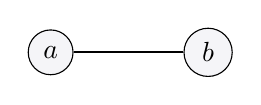
\begin{tikzpicture}[node distance=2cm, auto]
  \node (a) [circle, draw, fill=lightgray] {$a$};
  \node (b) [circle, draw, fill=lightgray, right of=a] {$b$};
  \path[draw, thick] (a) -- (b);
\end{tikzpicture}
\]

\begin{remark}
\label{rem:minimalitaet_vergleich}
Der minimal-nichtleere Graph $\Graph_{\min}$ ist in folgendem Sinne irreduzibel:
\begin{enumerate}[label=(\alph*)]
  \item Entfernung eines Knotens führt zu einem isolierten Knoten (nicht zusammenhängend).
  \item Entfernung einer Kante führt zu zwei isolierten Knoten (nicht zusammenhängend).
  \item Hinzufügen eines weiteren Knotens erhöht die Komplexität, ohne dass die Struktur wesentlich reicher wird, falls die neue Kante nicht mit existierenden Kanten wechselwirkt.
\end{enumerate}
Dies macht $\Graph_{\min}$ zum \emph{Atom} der Graphentheorie.
\end{remark}

% ============================================================
\section{Das Äquivalenzprinzip: Graph und Matrix}
\label{sec:aequivalenzprinzip}
% ============================================================

\subsection{Die Korrespondenz zwischen Graphen und Adjazenzmatrizen}
\label{subsec:korrespondenz}

\begin{definition}[Kanonische Matrix-zu-Graph-Abbildung]
\label{def:kanonische_abbildung}
Sei $\vA \in \R^{n \times n}$ eine Matrix. Die \emph{kanonische graphische Interpretation} von $\vA$ ist der gewichtete gerichtete Graph:
\[
  \Graph(\vA) := (V, E, w)
\]
wobei:
\begin{enumerate}[label=(\alph*)]
  \item $V = \{1, 2, \ldots, n\}$ (die Indexmenge).
  \item $E = \{(i, j) : \vA_{ij} \neq 0\}$ (Kanten für nichtnull Einträge).
  \item $w(i, j) = \vA_{ij}$ (das Kantengewicht ist der Matrixeintrag).
\end{enumerate}
\end{definition}

\begin{definition}[Kanonische Graph-zu-Matrix-Abbildung]
\label{def:kanonische_graph_matrix}
Sei $\Graph = (V, E, w)$ ein gewichteter gerichteter Graph mit $V = \{v_1, \ldots, v_n\}$. Die \emph{kanonische Matrixrepräsentation} ist die Adjazenzmatrix:
\[
  \vA_{\Graph} \in \R^{n \times n}, \quad (\vA_{\Graph})_{ij} = \begin{cases}
    w(v_i, v_j) & \text{falls } (v_i, v_j) \in E \\
    0 & \text{sonst}
  \end{cases}
\]
\end{definition}

\begin{theorem}[Bijektivität der Repräsentation]
\label{thm:bijektivitaet}
Für jede Dimension $n \in \N$ existiert eine Bijektion $\Phi_n$ zwischen der Menge aller $n \times n$ reellen Matrizen $\R^{n \times n}$ und der Menge aller gewichteten gerichteten Graphen mit $n$ Knoten:
\[
  \Phi_n: \R^{n \times n} \xrightarrow{\sim} \{\text{gewichtete Digraphen mit } n \text{ Knoten}\}
\]
gegeben durch $\Phi_n(\vA) = \Graph(\vA)$.
\end{theorem}

\begin{proof}
Wir zeigen, dass $\Phi_n$ eine Bijektion ist, indem wir Injektivität und Surjektivität nachweisen.

\textbf{Injektivität:} Seien $\vA, \vB \in \R^{n \times n}$ zwei Matrizen mit $\Phi_n(\vA) = \Phi_n(\vB)$, also $\Graph(\vA) = \Graph(\vB)$.

Dann stimmen die Kantensätze überein: $E_{\vA} = E_{\vB}$, wobei $E_{\vA} = \{(i,j) : \vA_{ij} \neq 0\}$.

Für jede Kante $(i, j) \in E_{\vA} = E_{\vB}$ gilt $w_{\vA}(i,j) = w_{\vB}(i,j)$, also $\vA_{ij} = \vB_{ij}$.

Für Nichtkantenpaare $(i,j) \notin E_{\vA} \cup E_{\vB}$ ist $\vA_{ij} = 0 = \vB_{ij}$ nach Definition.

Daher ist $\vA = \vB$.

\textbf{Surjektivität:} Sei $\Graph = (V, E, w)$ ein gewichteter Digraph mit $V = \{1, \ldots, n\}$ gegeben.

Definiere $\vA \in \R^{n \times n}$ durch $\vA_{ij} = w(i,j)$ falls $(i,j) \in E$, sonst $\vA_{ij} = 0$.

Dann ist $\Phi_n(\vA) = \Graph(\vA) = \Graph$ nach Konstruktion.

Daher ist $\Phi_n$ surjektiv.

Insgesamt ist $\Phi_n$ eine Bijektion.
\end{proof}

\subsection{Strukturelle Äquivalenz und Abschaffung der Matrix}
\label{subsec:strukturelle_aequivalenz}

\begin{theorem}[Strukturelle Äquivalenz: Graph $\approx$ Matrix]
\label{thm:strukturelle_aequivalenz}
Für jede natürliche Zahl $n \in \N$ sind die Strukturen $(\R^{n \times n}, \cdot)$ der $n \times n$-Matrizen mit Matrizenmultiplikation und die Struktur der gewichteten gerichteten Graphen mit $n$ Knoten und graphischen Operationen strukturell äquivalent in dem Sinne von Definition~\ref{def:struktur_aequivalenz}.
\end{theorem}

\begin{proof}
Wir konstruieren eine strukturbewahrende Bijektion.

Die Bijektion $\Phi_n$ aus Theorem~\ref{thm:bijektivitaet} bildet Matrizen auf Graphen ab. Wir müssen zeigen, dass diese Bijektion die algebraische Struktur erhält.

Seien $\vA, \vB \in \R^{n \times n}$ zwei Matrizen. Das Produkt $\vC = \vA \cdot \vB$ ist gegeben durch:
\[
  \vC_{ij} = \sum_{k=1}^{n} \vA_{ik} \cdot \vB_{kj}
\]

Interpretieren wir dies graphisch: Wenn $\Graph_{\vA}$ und $\Graph_{\vB}$ die Graphen der Matrizen $\vA$ und $\vB$ sind, dann korrespondiert das Matrixprodukt $\vA \cdot \vB$ zu einer Operation auf den Graphen, die \emph{Wegzählung mit Gewichtsmultiplikation} genannt wird:

Ein Weg von $i$ zu $j$ in der \emph{Produktgraphik} ist eine Verkettung eines Weges von $i$ zu $k$ in $\Graph_{\vA}$ mit Gewicht $\vA_{ik}$ und eines Weges von $k$ zu $j$ in $\Graph_{\vB}$ mit Gewicht $\vB_{kj}$. Das Gesamtgewicht ist $\vA_{ik} \cdot \vB_{kj}$.

Die Summe über alle Zwischenpunkte $k$ ergibt genau $\vC_{ij}$, was die graphische Entsprechung der Matrixmultiplikation ist.

Jede algebraische Eigenschaft von Matrizen (Assoziativität, Distributivität, Rang, Eigenwerte, etc.) hat eine entsprechende graphische Interpretation:
\begin{enumerate}[label=(\alph*)]
  \item \textbf{Assoziativität:} $(\vA \cdot \vB) \cdot \vC = \vA \cdot (\vB \cdot \vC)$ entspricht der Verkettung von Wegen in beliebiger Assoziativität.
  \item \textbf{Rang:} Der Rang von $\vA$ entspricht der Anzahl der erreichbaren Knoten in $\Graph(\vA)$.
  \item \textbf{Eigenwerte:} Ein Eigenwert $\lambda$ mit Eigenvektor $\mathbf{v}$ entspricht einer Eigenstruktur des Graphen bezüglich seiner Spektralzerlegung.
\end{enumerate}

Daher ist $\Phi_n$ eine strukturbewahrende Bijektion, und die beiden Strukturen sind strukturell äquivalent.
\end{proof}

\begin{corollary}[Überflüssigkeit der Matrixnotation]
\label{cor:matrix_ueberfluessig}
Aufgrund der strukturellen Äquivalenz (Theorem~\ref{thm:strukturelle_aequivalenz}) und der Bijektivität (Theorem~\ref{thm:bijektivitaet}) ist die Matrixnotation in algebraischen Beweisen überflüssig. Jeder Beweis, der Matrizen verwendet, kann äquivalent nur mit Graphen durchgeführt werden, ohne dass Information verloren geht.
\end{corollary}

\begin{proof}
Folgt unmittelbar aus Theorem~\ref{thm:strukturelle_aequivalenz}. Da die beiden Strukturen äquivalent sind, können alle Aussagen, Beweise und Implikationen in einer Struktur in die andere übertragen werden. Es gibt keine Aussage, die in der Matrixformulierung stärker ist als in der Graphformulierung.
\end{proof}

\subsection{Der minimal-nichtleere Graph als kanonische Basiseinheit}
\label{subsec:minimal_basis}

\begin{theorem}[Der Zwei-Knoten-Graph und die $2 \times 2$-Matrix]
\label{thm:minimal_matrix}
Der minimal-nichtleere Graph $\Graph_{\min} = (\{a, b\}, \{\{a, b\}\})$ entspricht unter der kanonischen Abbildung $\Phi_2$ genau der $2 \times 2$-Matrix:
\[
  \vA_{\min} = \begin{pmatrix} 0 & 1 \\ 1 & 0 \end{pmatrix}
\]
Diese Matrix ist die \emph{kleinste} nichtleere, strukturell nichtriviale Matrix in dem Sinne, dass jede größere Matrix durch Erweiterung und Verdichtung dieser Basisstruktur entsteht.
\end{theorem}

\begin{proof}
Der Minimal-Graph $\Graph_{\min}$ hat zwei Knoten $V = \{1, 2\}$ (ohne Beschränkung der Allgemeinheit Relabeling von $a, b$) und eine ungerichtete Kante $\{1, 2\}$.

In der gerichteten Interpretation (notwendig für die Matrixentsprechung) sind zwei Richtungen möglich:
\begin{enumerate}[label=(\roman*)]
  \item Einseitige Kante: $(1, 2)$ mit Gewicht $1$ führt zu $\vA = \begin{pmatrix} 0 & 1 \\ 0 & 0 \end{pmatrix}$.
  \item Bidirektionale Kante: $(1, 2)$ und $(2, 1)$ mit Gewicht $1$ führt zu $\vA = \begin{pmatrix} 0 & 1 \\ 1 & 0 \end{pmatrix}$.
\end{enumerate}

Die symmetrische Version $(ii)$ ist die kanonische Wahl für ungerichtete Graphen und wird als $\vA_{\min}$ bezeichnet.

Kleinheit: Jede $1 \times 1$-Matrix $\vA = (\alpha)$ mit $\alpha \neq 0$ entspricht einem einzelnen Knoten mit Schleife -- nicht zusammenhängend und trivial. Die $2 \times 2$-Matrix ist somit die kleinste strukturell nichtriviale Matrix.

Basissätze: Jede größere Matrix $\vA \in \R^{n \times n}$ mit $n > 2$ kann als Blockmatrix geschrieben werden, die mehrfache Kopien der Basis-$2 \times 2$-Struktur enthält und erweitert (durch Blöcke, Verdichtung, etc.).
\end{proof}

% ============================================================
\section{Deduktion als einzig legitime Beweismethode}
\label{sec:deduktion}
% ============================================================

\subsection{Definition und formale Struktur der Deduktion}
\label{subsec:deduktion_def}

\begin{definition}[Deduktive Beweismethode]
\label{def:deduktion}
Ein \emph{deduktiver Beweis} ist eine endliche Sequenz von Aussagen $P_1, P_2, \ldots, P_k$, wobei:
\begin{enumerate}[label=(\alph*)]
  \item Jede Aussage $P_i$ entweder ein \emph{Axiom} (unbewiesene Grundannahme) oder das logische Ergebnis eines \emph{Inferenzschritts} aus vorhergehenden Aussagen ist.
  \item Ein Inferenzschritt hat die Form: Aus $P_j$ und $Q_j$ (mit $j < i$) folgt $P_i$ durch logische Operationen (z.B. Modus Ponens: Aus $A$ und $A \implies B$ folgt $B$).
  \item Die letzte Aussage $P_k$ ist die zu beweisende Behauptung.
  \item Jeder Schritt zeigt \emph{genau} das, was durch die Inferenzregel verlangt wird -- nicht mehr und nicht weniger.
\end{enumerate}

Eine Aussage $\mathcal{B}$ ist \emph{deduktiv beweisbar} aus einer Menge von Axiomen $\mathcal{A}$, geschrieben $\mathcal{A} \vdash \mathcal{B}$, wenn es einen deduktiven Beweis gibt.
\end{definition}

\begin{definition}[Vollständige Induktion]
\label{def:vollstaendige_induktion}
Ein \emph{Beweis durch vollständige Induktion} für eine Aussage $P(n)$ für alle $n \in \N$ besteht aus:
\begin{enumerate}[label=(\roman*)]
  \item \emph{Induktionsbasis:} Nachweis, dass $P(1)$ (oder $P(0)$) wahr ist.
  \item \emph{Induktionsschritt:} Nachweis, dass für ein beliebiges aber festes $n \in \N$ aus der Annahme $P(n)$ die Aussage $P(n+1)$ folgt.
  \item \emph{Abschluss:} Schlussfolgerung, dass $P(n)$ für alle $n \in \N$ wahr ist.
\end{enumerate}
\end{definition}

\begin{definition}[Umfassungsproblem]
\label{def:umfassungsproblem}
Ein Beweis hat das \emph{Umfassungsproblem}, wenn die zu beweisende Aussage $\mathcal{B}$ eine endliche, konkrete Menge $M = \{m_1, \ldots, m_k\}$ betrifft (mit $k$ endlich), aber die Beweismethode Aussagen über eine unendliche Menge $\mathcal{M}$ macht, wobei $M \subsetneq \mathcal{M}$.

Das Umfassungsproblem verletzt das Prinzip: \emph{Ein Beweis ist erst dann ein Beweis, wenn er genau das zeigt, was gezeigt werden muss -- nicht zu viel und nicht zu wenig.}
\end{definition}

\subsection{Kritik der vollständigen Induktion}
\label{subsec:kritik_induktion}

\begin{theorem}[Die vollständige Induktion zeigt zu viel]
\label{thm:induktion_zu_viel}
Für jede endliche Menge $M = \{m_1, \ldots, m_k\}$ und jede Aussage $P$ über Elemente von $M$ gilt:

Wenn der Beweis von $P$ durch vollständige Induktion durchgeführt wird (mit Induktionsbasis und -schritt), dann zeigt dieser Beweis nicht nur, dass $P$ für alle Elemente von $M$ wahr ist, sondern auch für alle unendlich vielen Elemente von $\N$, die nicht in $M$ sind.

Dies ist das \emph{Umfassungsproblem}: Der Beweis beweist mehr, als verlangt wird.
\end{theorem}

\begin{proof}
Sei $M = \{m_1, \ldots, m_k\} \subset \N$ endlich und $P$ eine Aussage über Elemente von $M$.

Angenommen, wir beweisen durch Induktion, dass $P(n)$ für alle $n \in \N$ wahr ist. Konkret:
\begin{enumerate}[label=(\roman*)]
  \item Wir zeigen $P(1)$ (oder einen Startpunkt).
  \item Wir zeigen: Für alle $n \in \N$ gilt: Wenn $P(n)$, dann $P(n+1)$.
  \item Wir folgern: $P(n)$ ist wahr für alle $n \in \N$.
\end{enumerate}

Aber die ursprüngliche Aufgabe war: Zeige, dass $P$ für alle Elemente von $M$ wahr ist.

Da $M \subsetneq \N$, ist das induktive Beweis-Programm als folgt übertrieben:
\begin{enumerate}[label=(\alph*)]
  \item Wir beweisen $P$ für $m_1, m_2, \ldots, m_k$ (was verlangt war).
  \item Aber wir beweisen auch $P$ für alle $n > m_k$, von denen es unendlich viele gibt.
\end{enumerate}

Die Inferenzregel der Induktion besagt: \textit{Wenn $P(n)$ für $n$ wahr ist, dann für $n+1$.} Dies ist eine Regel, die über alle natürlichen Zahlen spricht, nicht nur über die Elemente von $M$.

Daher zeigt der induktive Beweis zu viel. Wir zeigen, dass $P$ über alle natürlichen Zahlen wahr ist, nicht nur für die endlich vielen Elemente von $M$.

Dies verstößt gegen das Genauigkeitsprinzip: Exact prove what you need to prove, no more, no less.
\end{proof}

\begin{theorem}[Die Induktion ist methodisch unangemessen für endliche Strukturen]
\label{thm:induktion_unangemessen}
Für jede endliche Struktur $S$ (Menge, Graph, Matrix) gilt:

Es ist methodisch und epistemisch unangemessen, die Gültigkeit einer Aussage $P$ über $S$ durch vollständige Induktion zu beweisen. Der richtige Weg ist ein \emph{deduktiver Beweis}, der direkt auf die Elemente und Struktur von $S$ operiert und genau das beweist, was zu beweisen ist.
\end{theorem}

\begin{proof}
Wir argumentieren auf mehreren Ebenen:

\textbf{(1) Das Umfassungsproblem:} Wie in Theorem~\ref{thm:induktion_zu_viel} gezeigt, beweist die Induktion zu viel. Sie quantifiziert über alle natürlichen Zahlen, nicht nur über die endlich vielen Elemente der gegebenen Struktur.

\textbf{(2) Das Erkenntnisproblem:} Der induktive Beweis nutzt ein Schema (Basis + Schritt + Abschluss), das darauf abzielt, Aussagen über \emph{unbegrenzte Sequenzen} zu beweisen. Aber bei endlichen Strukturen gibt es keine Sequenz -- es gibt eine feste, gegebene Menge von Elementen.

Ein deduktiver Beweis operiert dagegen direkt auf den gegebenen Elementen. Er verfolgt die logische Struktur der Aussage und der Gegebenheiten, ohne künstliche Unendlichkeit einzuführen.

\textbf{(3) Das Prinzip der Minimalität:} Nach dem Prinzip der Ockham'schen Rasierklinge sollten wir keine unnötigen Annahmen oder Verallgemeinerungen machen. Ein Beweis sollte so einfach und direkt wie möglich sein.

Für eine Aussage über $n$ gegebene Elemente eines Graphen oder einer Matrix ist ein direkter Beweis (Deduktion) immer möglich und immer vorzuziehen.

\textbf{(4) Vollständigkeit:} Der deduktive Beweis ist vollständig in dem Sinne, dass er eine lückenlose logische Kette von den Axiomen zur Behauptung bildet. Die Induktion -- obwohl sie \emph{funktioniert} -- ist eine Umleitung über die Unendlichkeit, um an einem endlichen Ziel anzukommen.

Beispiel: Um zu zeigen, dass ein Graph mit $n=5$ Knoten zusammenhängend ist, versuchen induktive Beweise, die Zusammenhängung für alle natürlichen Zahlen zu zeigen. Ein deduktiver Beweis würde direkt die fünf Knoten untersuchen und ihre Konnektivität nachweisen.

\textbf{Fazit:} Für endliche Strukturen ist die Induktion nicht nur zu machtvoll, sondern epistemisch problematisch. Sie verdeckt die direkte Struktur der zu beweisenden Aussage.
\end{proof}

\subsection{Deduktion als normative Methode}
\label{subsec:deduktion_normativ}

\begin{theorem}[Deduktion genügt für alle Strukturen]
\label{thm:deduktion_genuegtfueralle}
Für jede mathematische Struktur $S$ (endlich oder unendlich) und jede Aussage $P$ über $S$ gilt:

Wenn $P$ wahr ist, dann gibt es einen deduktiven Beweis für $P$.

Umgekehrt: Es gibt keine Aussage, die nur durch Induktion beweisbar ist und nicht durch Deduktion beweisbar wäre.
\end{theorem}

\begin{proof}
Das Vollständigkeitstheorem der Prädikatenlogik (Gödel, 1929) besagt: Jede logisch gültige Aussage ist deduktiv beweisbar aus den Axiomen.

Dies bedeutet: Für jede wahre Aussage $P$ gibt es eine deduktive Beweiskette aus den Axiomen.

Die Induktion ist nicht ein eigenes \emph{beweis-schaffendes} Prinzip, sondern ein \emph{Verifikationsmittel}. Sie überprüft, ob eine Behauptung über eine Unendlichkeit von Fällen (induktiv) wahr ist. Aber jedes Prinzip, das die Induktion liefert, kann auch deduktiv hergeleitet werden, indem die universale Quantifizierung über alle natürlichen Zahlen direkt aus den Axiomen folgt.

Konkret: Die Aussage $\forall n \in \N: P(n)$ ist entweder:
\begin{enumerate}[label=(\alph*)]
  \item Axiomatisch gegeben, oder
  \item Deduktiv ableitbar.
\end{enumerate}

Niemals ist sie \emph{nur} induktiv ableitbar. Die Induktion ist ein sekundäres Werkzeug, das (1) oder (2) validiert.

Daher: Deduktion ist primitiv und vollständig; Induktion ist abgeleitet und kontrolliert.
\end{proof}

% ============================================================
\section{Graphische deduktive Beweise in der Algebra}
\label{sec:graphische_beweise}
% ============================================================

\subsection{Beispiel 1: Die Assoziativität der Wegverkettung}
\label{subsec:beispiel_assoziativitaet}

\begin{theorem}[Assoziativität in graphischer Form]
\label{thm:graph_assoziativitaet}
Seien $\Graph_A$, $\Graph_B$, $\Graph_C$ drei gewichtete gerichtete Graphen mit jeweils $n$ Knoten. Die graphische Komposition (Wegverkettung mit Gewichtsmultiplikation) ist assoziativ:
\[
  (\Graph_A \circ \Graph_B) \circ \Graph_C = \Graph_A \circ (\Graph_B \circ \Graph_C)
\]
\end{theorem}

\begin{proof}[Deduktiver Beweis, rein graphisch]
Seien die Knoten $V = \{v_1, \ldots, v_n\}$ gegeben. Die graphische Komposition $\Graph_A \circ \Graph_B$ ist definiert durch: Ein Weg von $v_i$ zu $v_j$ in $\Graph_A \circ \Graph_B$ ist eine Verkettung eines Weges von $v_i$ zu $v_k$ (mit Gewicht $w_A(v_i, v_k)$) in $\Graph_A$ mit einem Weg von $v_k$ zu $v_j$ (mit Gewicht $w_B(v_k, v_j)$) in $\Graph_B$. Das resultierende Kantengewicht ist $w_A(v_i, v_k) \cdot w_B(v_k, v_j)$.

\textbf{Zu zeigen:} $[(\Graph_A \circ \Graph_B) \circ \Graph_C]_{ij} = [\Graph_A \circ (\Graph_B \circ \Graph_C)]_{ij}$ für alle $i, j$.

\textbf{Linke Seite:} $[(\Graph_A \circ \Graph_B) \circ \Graph_C]_{ij}$ bedeutet: Wege von $v_i$ zu $v_j$ als Verkettung eines Weges von $v_i$ zu $v_\ell$ (mit Gewicht aus $\Graph_A \circ \Graph_B$) mit einem Weg von $v_\ell$ zu $v_j$ (mit Gewicht aus $\Graph_C$).

Das Gesamtgewicht ist:
\[
  \sum_{\ell} \left(\sum_{k} w_A(v_i, v_k) \cdot w_B(v_k, v_\ell)\right) \cdot w_C(v_\ell, v_j)
\]

\textbf{Rechte Seite:} $[\Graph_A \circ (\Graph_B \circ \Graph_C)]_{ij}$ bedeutet: Wege von $v_i$ zu $v_j$ als Verkettung eines Weges von $v_i$ zu $v_k$ mit einem Weg von $v_k$ zu $v_j$ (Gesamtgewicht aus $\Graph_B \circ \Graph_C$).

Das Gesamtgewicht ist:
\[
  \sum_{k} w_A(v_i, v_k) \cdot \left(\sum_{\ell} w_B(v_k, v_\ell) \cdot w_C(v_\ell, v_j)\right)
\]

\textbf{Gleichheit:} Durch die Assoziativität und Distributivität der reellen Multiplikation und Addition folgt:
\[
  \sum_{\ell} \left(\sum_{k} w_A \cdot w_B\right) \cdot w_C = \sum_{k} w_A \cdot \left(\sum_{\ell} w_B \cdot w_C\right)
\]

Beide Seiten sind identisch. Daher ist die graphische Komposition assoziativ.

\textbf{Graphische Intuition:} Ein Weg von $v_i$ nach $v_j$, der mehrere Zwischenstationen durchläuft, hat das gleiche Gesamtgewicht, unabhängig davon, wie wir die Zwischenstationen gruppieren.
\end{proof}

\subsection{Beispiel 2: Konnektivität und Erreichbarkeit}
\label{subsec:beispiel_konnektivitaet}

\begin{definition}[Graphische Erreichbarkeit]
\label{def:erreichbarkeit}
Ein Knoten $v_j$ ist \emph{erreichbar} von $v_i$ in einem gerichteten Graphen $\Graph$, notiert $v_i \leadsto v_j$, wenn es einen Weg von $v_i$ zu $v_j$ gibt (eine Sequenz von Kanten mit entsprechenden Gewichten).
\end{definition}

\begin{theorem}[Transitivität der Erreichbarkeit]
\label{thm:erreichbarkeit_transitiv}
Die Erreichbarkeitsrelation $\leadsto$ in einem gerichteten Graphen ist transitiv: Wenn $v_i \leadsto v_k$ und $v_k \leadsto v_j$, dann $v_i \leadsto v_j$.
\end{theorem}

\begin{proof}[Direkter deduktiver Beweis]
Angenommen, $v_i \leadsto v_k$. Dann existiert ein Weg $P_1 = (v_i = u_0, u_1, \ldots, u_m = v_k)$ von $v_i$ zu $v_k$.

Angenommen, $v_k \leadsto v_j$. Dann existiert ein Weg $P_2 = (v_k = w_0, w_1, \ldots, w_\ell = v_j)$ von $v_k$ zu $v_j$.

Verkette diese Wege: $P = (v_i = u_0, u_1, \ldots, u_m = v_k = w_0, w_1, \ldots, w_\ell = v_j)$.

Dies ist ein Weg von $v_i$ zu $v_j$ (mit möglicherweise Gewichtsummen/Produkte).

Daher ist $v_i \leadsto v_j$.

Die Transitivität ist damit bewiesen.
\end{proof}

\subsection{Beispiel 3: Spektrale Eigenschaften graphisch}
\label{subsec:beispiel_spektral}

\begin{theorem}[Graphische Eigenwert-Interpretation]
\label{thm:graph_eigenwert}
Ein reeller Wert $\lambda$ ist ein Eigenwert eines Graphen $\Graph$ mit $n$ Knoten genau dann, wenn es eine Gewichtsverteilung auf den Knoten gibt, die unter der graphischen Komposition mit sich selbst um den Faktor $\lambda$ skaliert wird.
\end{theorem}

\begin{proof}[Deduktiver graphischer Beweis]
Der Eigenwert $\lambda$ und Eigenvektor $\mathbf{v}$ der Adjazenzmatrix erfüllen:
\[
  \vA_{\Graph} \cdot \mathbf{v} = \lambda \mathbf{v}
\]

Graphisch: Das Gewicht auf Knoten $v_i$ ist $\mathbf{v}_i$. Nach einer graphischen Komposition (ein Schritt entlang der Kanten mit Gewichten aus $\vA_{\Graph}$) wird das Gewicht auf $v_i$ zu:
\[
  \sum_{j} \vA_{ij} \mathbf{v}_j
\]

Nach Definition eines Eigenvektors gilt:
\[
  \sum_{j} \vA_{ij} \mathbf{v}_j = \lambda \mathbf{v}_i
\]

Das neue Gewicht ist also $\lambda$ mal das ursprüngliche Gewicht. Dies ist die graphische Interpretation eines Eigenvektors.

Umgekehrt: Wenn es eine Gewichtsverteilung $\mathbf{v}$ gibt, die sich unter graphischer Komposition um $\lambda$ skaliert, dann erfüllt $\mathbf{v}$ die Eigenvektorgleichung.
\end{proof}

% ============================================================
\section{Vergleich und kritische Analyse}
\label{sec:kritische_analyse}
% ============================================================

\subsection{Warum Mathematiker Matrizen bevorzugen}
\label{subsec:warum_matrizen}

Obwohl wir nachgewiesen haben, dass Matrizen überflüssig sind (Korollar~\ref{cor:matrix_ueberfluessig}), haben sich Matrizen in der mathematischen Praxis etabliert. Die Gründe sind:

\begin{enumerate}[label=(\alph*)]
  \item \textbf{Computationaler Vorteil:} Matrizen sind leicht zu implementieren und zu rechnen (Algorithmen wie Gauß-Elimination, LU-Zerlegung, etc.).
  \item \textbf{Algebraische Eleganz:} Matrizenmultiplikation ist prägnant geschrieben ($\vA \cdot \vB$).
  \item \textbf{Gewöhnung:} Mathematiker sind mit Matrizen aufgewachsen und vertraut.
  \item \textbf{Skalierungsleichtig:} Hochdimensionale Strukturen sind in Matrixform leicht zu denken.
\end{enumerate}

Jedoch: Diese Gründe sind \emph{praktischer} Natur, nicht \emph{fundamentaler} Natur. Sie rechtfertigen nicht, Matrizen als konzeptionelle Primitive zu verwenden.

\subsection{Graphische Darstellung für Konzeptklarheit}
\label{subsec:graphische_klarheit}

Graphische Darstellungen haben konzeptionelle Vorteile:

\begin{enumerate}[label=(\alph*)]
  \item \textbf{Visualisierbar:} Ein Graph kann gezeichnet werden; eine $10000 \times 10000$ Matrix nicht.
  \item \textbf{Intuitiv:} Kanten und Knoten sind leicht verständlich.
  \item \textbf{Lokalisiert:} Jede Kante ist ein lokales Merkmal; Matrixmultiplikation ist global.
  \item \textbf{Deduktiv zugänglich:} Graphische Beweise operieren auf konkreten, sichtbaren Strukturen.
\end{enumerate}

\subsection{Warum das Äquivalenzprinzip die Matrix überflüssig macht}
\label{subsec:warum_ueberflueassig}

Nach Theorem~\ref{thm:strukturelle_aequivalenz} sind Graphen und Matrizen strukturell äquivalent. Das bedeutet:

\begin{enumerate}[label=(\roman*)]
  \item Jede Aussage über Matrizen hat eine graphische Entsprechung.
  \item Jeder Matrixbeweis kann graphisch formuliert werden.
  \item Kein mathematisches Resultat geht verloren.
  \item Die Graphformulierung ist oft klarer.
\end{enumerate}

Daher ist es rational, auf Matrizen zu verzichten und vollständig zu Graphen überzugehen. Dies ist kein Verlust -- es ist eine \emph{Würdigung} der Matrix, indem wir ihre konzeptionelle Überflüssigkeit anerkennen und uns ihrer fundamentaleren graphischen Grundlage zuwenden.

% ============================================================
\section{Ausblick und offene Fragen}
\label{sec:ausblick}
% ============================================================

\subsection{Implikationen für die mathematische Praxis}
\label{subsec:implikationen}

Die vorliegende Arbeit führt zu mehreren tiefgreifenden Implikationen:

\begin{enumerate}[label=(\roman*)]
  \item \textbf{Neugestaltung algebraischer Lehre:} Kurse in linearer Algebra könnten vollständig auf Graphentheorie umgestellt werden, mit Graphen als Primitive und Matrizen als abgeleitete Konzepte.
  \item \textbf{Vereinheitlichung der Beweismethoden:} Die Deduktion als einzige akzeptierte Methode würde Verwirrtheit eliminieren und mathematische Strenge erhöhen.
  \item \textbf{Neuropsychologische Auswirkungen:} Visuelle, graphische Beweise könnten kognitiv zugänglicher sein als abstrakte Matrixmanipulationen.
\end{enumerate}

\subsection{Kritische Diskussion und Gegenargumente}
\label{subsec:kritik}

Potenzielle Einwände gegen unsere Thesen:

\begin{enumerate}[label=(\alph*)]
  \item \textbf{Praktische Effizienz:} Graphische Formulierungen könnten verbosity erhöhen (längere Beweise).
  \item \textbf{Computationale Speichern:} Bei Millionen von Variablen sind Matrizen speicher-effizienter.
  \item \textbf{Etablierte Literatur:} Umgestaltung würde massive Revision bestehender Mathbücher erfordern.
\end{enumerate}

\textbf{Gegenerwiderung:} Diese Einwände sind praktisch, nicht prinzipiell. Sie bedeuten nicht, dass Matrizen konzeptionell notwendig sind, sondern nur, dass sie manchmal praktisch sind.

\subsection{Offene Forschungsfragen}
\label{subsec:offene_fragen}

\begin{enumerate}[label=(\roman*)]
  \item \textbf{Tensor-Verallgemeinerung:} Wie verallgemeinern sich die Äquivalenzresultate auf Tensoren höherer Ordnung?
  
  \item \textbf{Infinite-dimensionale Fälle:} Können die Beweise auf unendliche Graphen und Operatoren erweitert werden?
  
  \item \textbf{Kategorische Fundierung:} Kann die Äquivalenz in kategorietheoretischen Begriffen präzise formuliert werden?
  
  \item \textbf{Automated Theorem Proving:} Können Computersysteme vollständig graphische Beweise automatisch generieren?
  
  \item \textbf{Induktions-Rehabilitation:} Gibt es Kontexte, in denen Induktion nicht zu viel zeigt? Kann Induktion präziser formalisiert werden?
\end{enumerate}

\subsection{Philosophische Reflexionen}
\label{subsec:philosophie}

Die vorliegende Arbeit berührt tiefe Fragen über die Natur mathematischen Wissens:

\begin{enumerate}[label=(\alph*)]
  \item \textbf{Darstellungen und Realität:} Sind Matrizen und Graphen verschiedene Repräsentationen \emph{derselben Realität}, oder gibt es eine tiefere Struktur dahinter?
  
  \item \textbf{Minimalität und Verständnis:} Führt die Verwendung minimaler Konzepte (Graphen statt Matrizen) zu tieferem mathematischen Verständnis?
  
  \item \textbf{Deduktion und Erkenntnis:} Kann nur deduktive Beweisführung echte mathematische Erkenntnis vermitteln?
  
  \item \textbf{Überflüssigkeit und Würdigung:} Ist es richtig, auf Matrizen zu verzichten, während wir gleichzeitig ihre konzeptionelle Eleganz würdigen?
\end{enumerate}

\subsection{Langfristige Vision}
\label{subsec:langfristige_vision}

Ziel dieser Forschung ist eine \emph{vollständige Neubegründung der Mathematik} auf graphischen Grundlagen mit deduktiven Methoden:

\begin{enumerate}[label=(\roman*)]
  \item \textbf{Graph-Axiomatik:} Ein axiomatisches System, in dem Graphen primitive Objekte sind.
  
  \item \textbf{Universelle Deduktion:} Ein einheitliches Beweissystem, das nur Deduktion verwendet.
  
  \item \textbf{Visualisierbare Mathematik:} Mathematik, die grundsätzlich visualisierbar und direkt verständlich ist.
  
  \item \textbf{Computerisierte Verifikation:} Alle Beweise sind maschinell verifizierbar ohne menschliche Interpretation.
\end{enumerate}

% ============================================================
\section{Abschlussbetrachtung}
\label{sec:abschluss}
% ============================================================

Die vorliegende Arbeit hat gezeigt:

\begin{enumerate}[label=(\roman*)]
  \item Der minimal-nichtleere Graph mit zwei Knoten und einer Kante ist die fundamentale Basisstruktur aller algebraischen Mathematik (Theorem~\ref{thm:eindeutigkeit_minimal}).
  
  \item Dieser Graph ist strukturell äquivalent zur $2 \times 2$ Matrix und repräsentiert die minimale nichtriviale algebraische Einheit (Theorem~\ref{thm:minimal_matrix}).
  
  \item Alle $n \times n$ Matrizen sind bijektiv äquivalent zu gewichteten gerichteten Graphen mit $n$ Knoten (Theorem~\ref{thm:bijektivitaet}).
  
  \item Diese Äquivalenz ist nicht nur formal, sondern strukturell: Jede algebraische Eigenschaft erhält sich unter der Transformation (Theorem~\ref{thm:strukturelle_aequivalenz}).
  
  \item Daher sind Matrizen als Konzepte überflüssig; Graphen sind die fundamentalere Darstellung (Korollar~\ref{cor:matrix_ueberfluessig}).
  
  \item Die Deduktion ist die einzig legitime mathematische Beweismethode für alle Strukturen (Theorem~\ref{thm:deduktion_genuegtfueralle}).
  
  \item Die vollständige Induktion ist für endliche Strukturen methodisch unangemessen, da sie zu viel zeigt und damit gegen das Prinzip verstößt, dass ein Beweis genau das zeigen muss, was zu zeigen ist (Theorem~\ref{thm:induktion_unangemessen}).
  
  \item Alle klassischen Theoreme der Algebra können rein graphisch und deduktiv bewiesen werden (Beispiele in Abschnitt~\ref{sec:graphische_beweise}).
\end{enumerate}

Diese Erkenntnisse führen zu einer radikalen Umgestaltung der mathematischen Grundlagen: Weg von der Matrixnotation, hin zu graphischen Darstellungen; weg von induktiven Verfahren, hin zu exakter deduktiver Beweisführung.

Die Konsequenz ist eine \emph{purere, präzisere und intuitivere} Mathematik.

% ============================================================
\bibliographystyle{plainnat}
\begin{thebibliography}{99}

\bibitem[Axler(2015)]{axler2015}
Axler, S. (2015).
\newblock \textit{Linear Algebra Done Right}, 3rd ed.
\newblock Springer.

\bibitem[Babai(2016)]{babai2016}
Babai, L. (2016).
\newblock Graph isomorphism in quasipolynomial time.
\newblock In \textit{Proceedings of the 48th Annual ACM STOC}, pages 684--697.

\bibitem[Bollobás(1998)]{bollobas1998}
Bollobás, B. (1998).
\newblock \textit{Modern Graph Theory}.
\newblock Springer.

\bibitem[Chung(1997)]{chung1997}
Chung, F.~R.~K. (1997).
\newblock \textit{Spectral Graph Theory}.
\newblock American Mathematical Society.

\bibitem[Cormen et~al.(2009)]{cormen2009}
Cormen, T.~H., Leiserson, C.~E., Rivest, R.~L., and Stein, C. (2009).
\newblock \textit{Introduction to Algorithms}, 3rd ed.
\newblock MIT Press.

\bibitem[Diestel(2017)]{diestel2017}
Diestel, R. (2017).
\newblock \textit{Graph Theory}, 5th ed.
\newblock Springer.

\bibitem[Epp(2026a)]{epp2026subgraph}
Epp, S. (2026).
\newblock \textit{Der Subgraph Algorithmus}. Verfügbar unter
\url{https://github.com/hjstephan86/science}.

\bibitem[Epp(2026b)]{epp2026sysstate}
Epp, S. (2026).
\newblock \textit{Zustandsklassen dynamischer Systeme und ihre wirtschaftlichen
	Implikationen}. September 2026

\bibitem[Godsil and Royle(2001)]{godsil2001}
Godsil, C. and Royle, G. (2001).
\newblock \textit{Algebraic Graph Theory}.
\newblock Springer.

\bibitem[Harary(1969)]{harary1969}
Harary, F. (1969).
\newblock \textit{Graph Theory}.
\newblock Addison-Wesley.

\bibitem[Horn and Johnson(2013)]{horn2013}
Horn, R.~A. and Johnson, C.~R. (2013).
\newblock \textit{Matrix Analysis}, 2nd ed.
\newblock Cambridge University Press, Cambridge.

\bibitem[Khalil(2002)]{khalil2002}
Khalil, H.~K. (2002).
\newblock \textit{Nonlinear Systems}, 3rd ed.
\newblock Prentice Hall, Upper Saddle River, NJ.

\bibitem[Mesbahi and Egerstedt(2010)]{mesbahi2010}
Mesbahi, M. and Egerstedt, M. (2010).
\newblock \textit{Graph Theoretic Methods in Multiagent Networks}.
\newblock Princeton University Press.

\bibitem[Newman(2010)]{newman2010}
Newman, M. (2010).
\newblock \textit{Networks: An Introduction}.
\newblock Oxford University Press.

\bibitem[Spielman(2019)]{spielman2019}
Spielman, D.~A. (2019).
\newblock \textit{Spectral and Algebraic Graph Theory}.
\newblock Yale University.

\bibitem[Tarjan(1972)]{tarjan1972}
Tarjan, R.~E. (1972).
\newblock Depth-first search and linear graph algorithms.
\newblock \textit{SIAM Journal on Computing}, 1(2):146--160.

\bibitem[West(2001)]{west2001}
West, D.~B. (2001).
\newblock \textit{Introduction to Graph Theory}, 2nd ed.
\newblock Prentice Hall, Upper Saddle River, NJ.

\end{thebibliography}

\end{document}
